\lstinputlisting[language=bash,basicstyle=\small]{python_codes/fieldstone_05/keywords}

\begin{center}
Code at \url{https://github.com/cedrict/fieldstone/tree/master/python_codes/fieldstone_05}
\end{center}

\par\noindent\rule{\textwidth}{0.4pt}
%%%%%%%%%%%%%%%%%%%%%%%%%%%%%%%%%%%%%%%%%%%%%%%%%%%%%%%%%%%%%%%%%%%%%%%%%%%%%%%%%%%%%%%%%

The experiment is fully described in Section~\ref{ss:solcx}.
The viscosity is prescribed at the quadrature points 
If the number of elements is even in the $x$-direction direction, all elements 
(and their associated quadrature points)
have a constant viscosity ($1$ or  $10^6$). If it is odd, then the elements situated 
at the viscosity jump have half their integration points with $\mu=1$ and half with $\mu=10^6$ 
(which is a pathological case since the used quadrature rule inside elements cannot represent 
accurately such a jump).  

\begin{center}
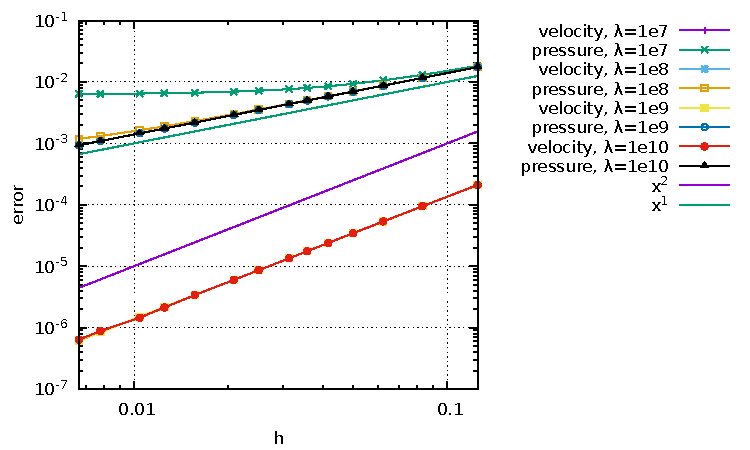
\includegraphics[width=7cm]{python_codes/fieldstone_05/results/errors_even.pdf}
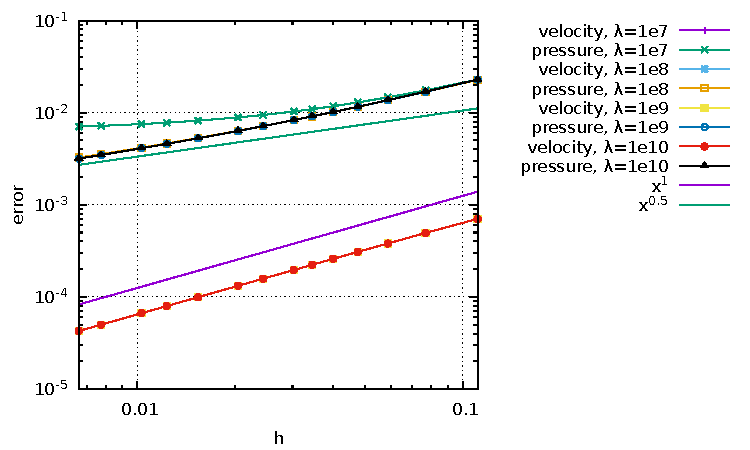
\includegraphics[width=7cm]{python_codes/fieldstone_05/results/errors_odd.pdf}\\
{\captionfont Velocity and pressure error convergence as a function of mesh size and for various values
of the penalty parameter. Left: even number of elements in each direction; Right: odd numbers.
}
\end{center}

Because of the high viscosity in the right part of the domain, the penalty parameter should 
be high enough to insure an incompressible flow and thereby recover the expected convergence rate
(at least for the even case). Note that values higher than $\lambda=10^{10}$ yield erroneous solutions 
due to round-off errors. 

\begin{center}
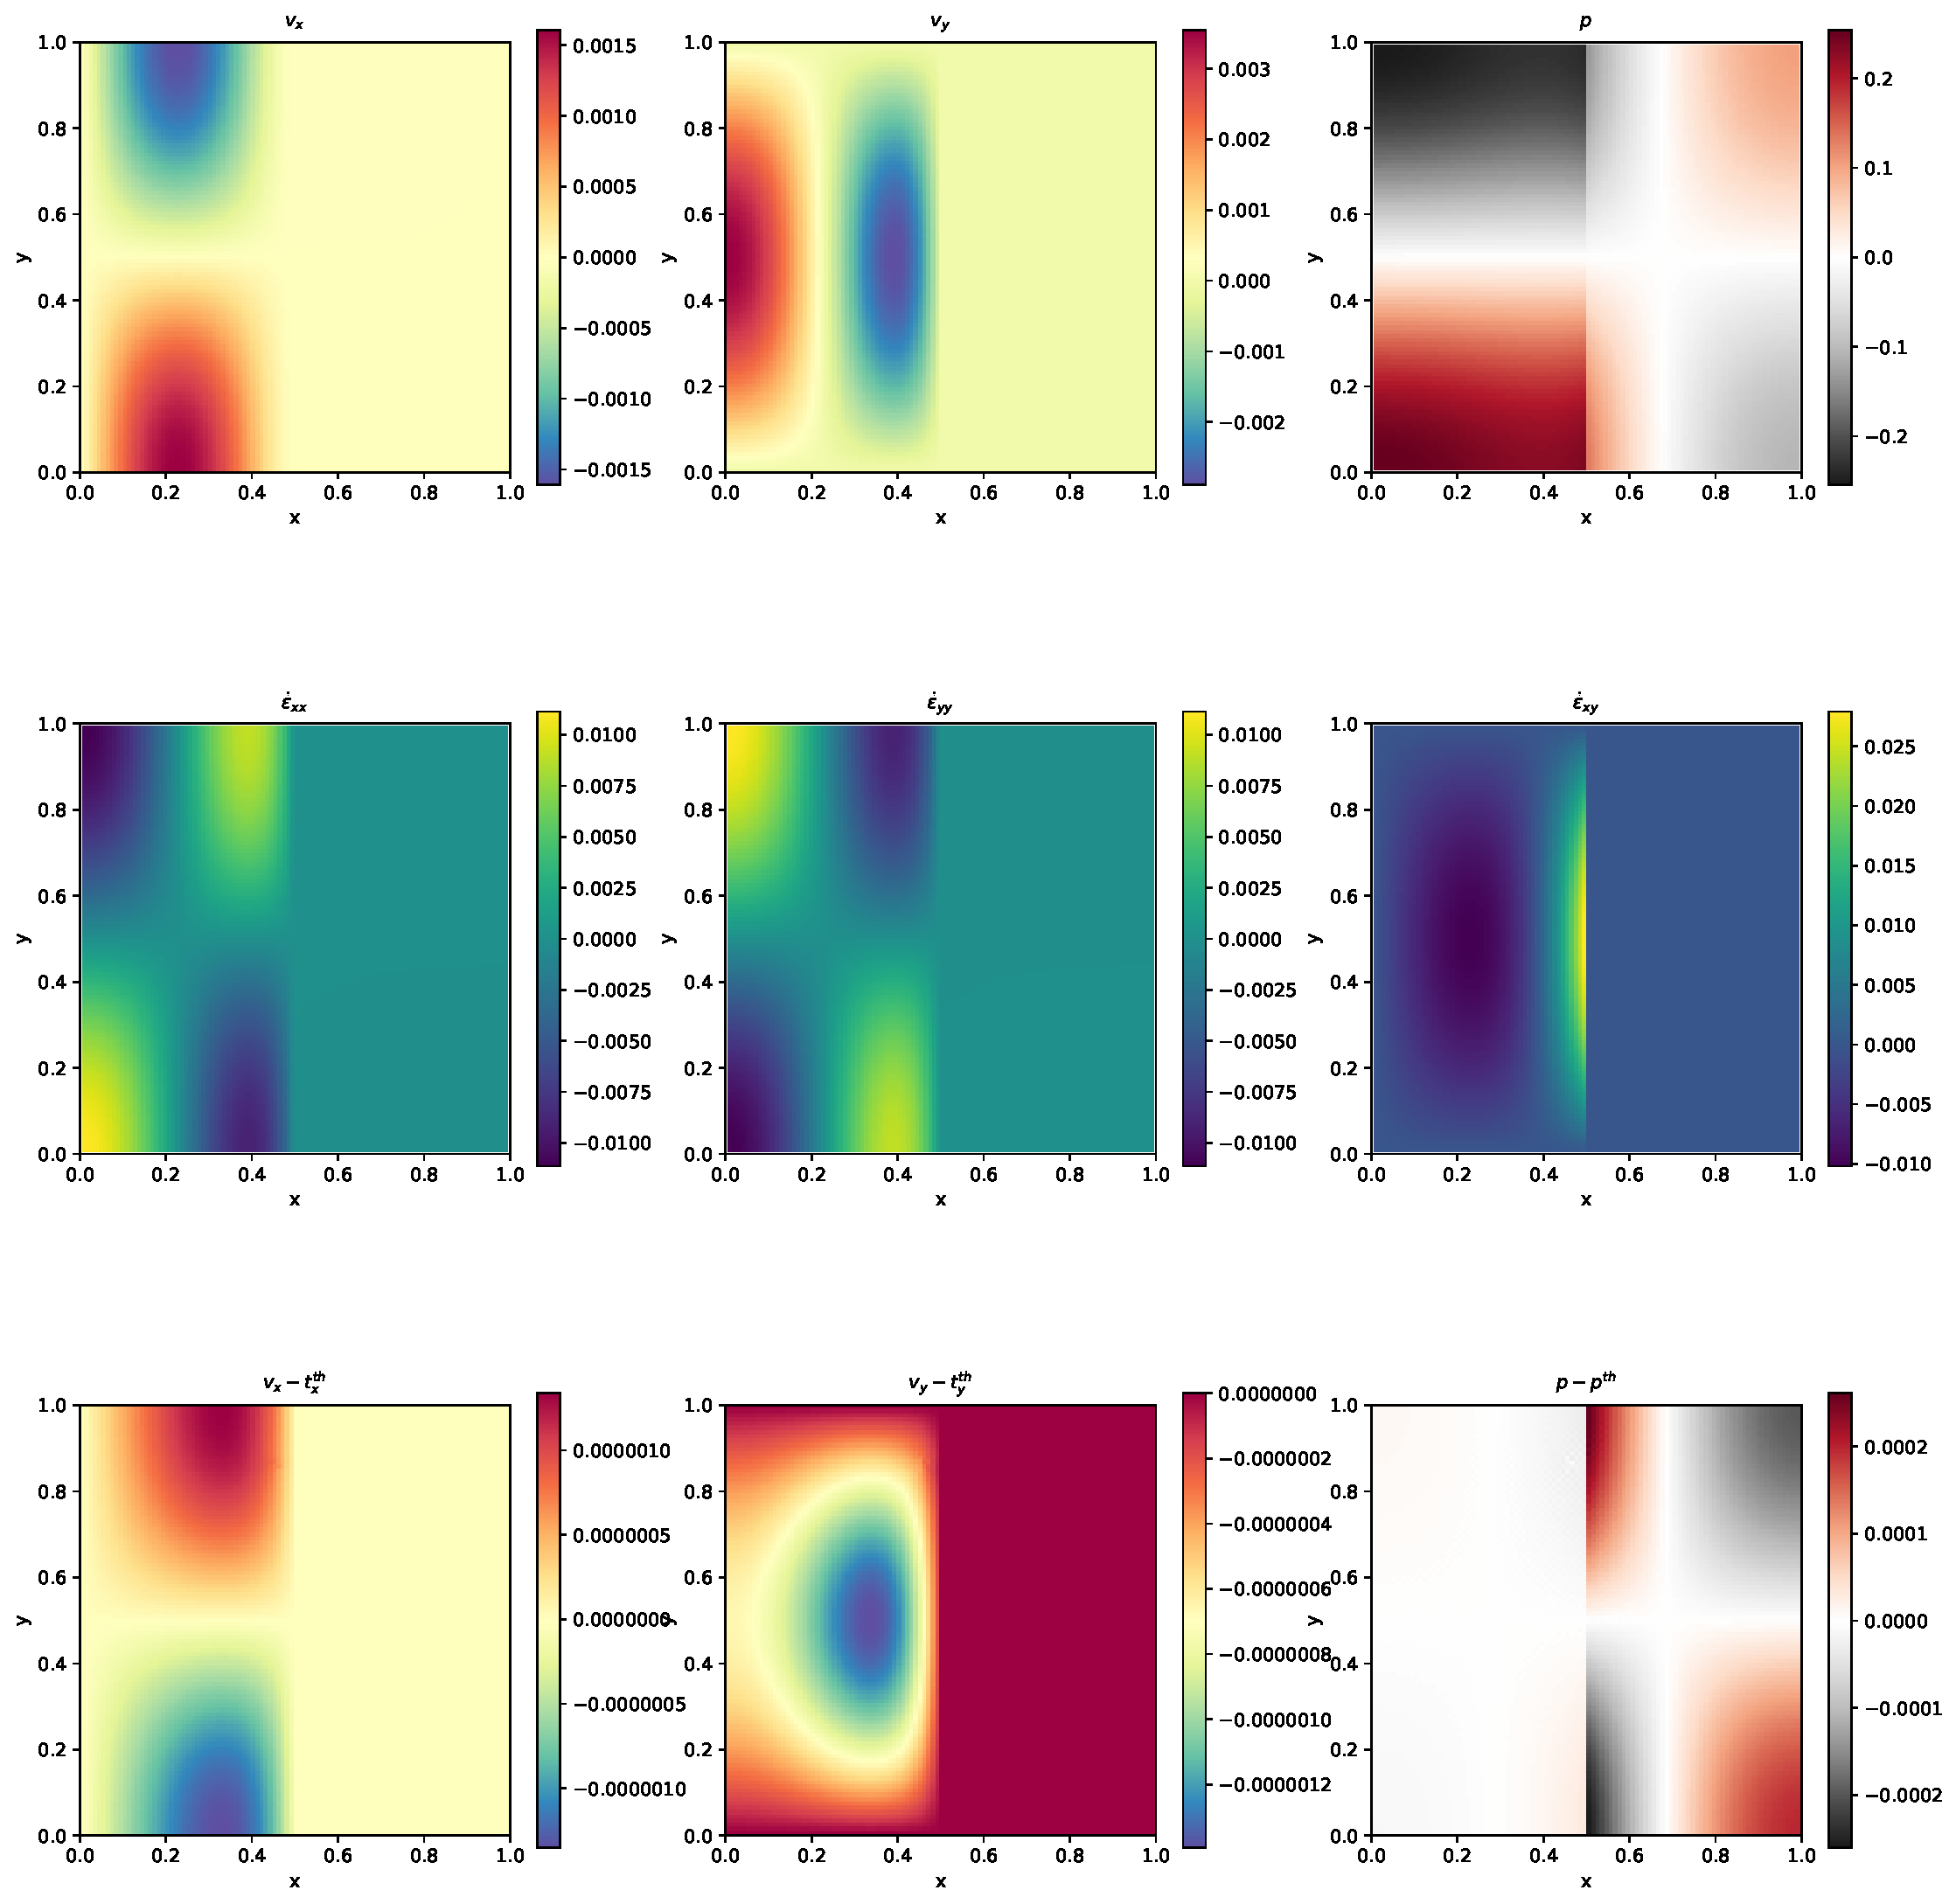
\includegraphics[width=16cm]{python_codes/fieldstone_05/results/solution.pdf}
{\captionfont Various fields for 100x100 mesh}
\end{center}

Note that a fortran version of this code is available in the same folder.


